%% SUMMARY OF COMPARISON CEAP - AFFECTIVE VR
% ----------------------------------------------------- set up ---------------------------------------------------------------
\documentclass[11pt, letterpaper]{article}
\usepackage{graphicx}
\graphicspath{/Users/Lucy/Documents/Berlin/FU/MCNB/Praktikum/MPI_MBE/AffectiveVR/Phase1/CEAP/results/}
\usepackage{caption}
\usepackage{subcaption}
\usepackage{hyperref}
\hypersetup{
    colorlinks=true,
    linkcolor=blue,
    filecolor=magenta,      
    urlcolor=cyan,
    pdftitle={comparison_ceap_affectivevr},
    pdfpagemode=FullScreen,
    }
\urlstyle{same}
\usepackage[utf8]{inputenc}
\usepackage{float}

% ----------------------------------------------------- title ---------------------------------------------------------------
\title{Comparison CEAP and AffectiveVR Phase 1}
\author{Lucy Roellecke}
\date{01 November 2023}
\begin{document}
\maketitle

% ----------------------------------------------------- abstract ---------------------------------------------------------------
\begin{abstract}
This document summarizes the results of performing a comparison of the \textit{Continuous Physiological and Behavioral Emotion Annotation Dataset for 360° Videos (CEAP-360VR}, available here: \url{https://github.com/cwi-dis/CEAP-360VR-Dataset}) and the data from phase 1 of our \textit{Affective VR} study. Both experiments were similar as in that they used 360° Virtual Reality (VR) videos with a length of 60 seconds each as stimulus material, and a continuous rating method based on the Circumplex Model of Emotion as affective measure. However, they differed in the exact nature of the rating method. Nonetheless, the results reported in this document support the assumption that both experiments elicit similar affective responses.
\end{abstract}

\newpage

% ----------------------------------------------------- analysis notes ---------------------------------------------------------------
\section{Analysis Notes}
In order to be able to compare both datasets, individual data from the CEAP study was first preprocessed using \verb|01_preprocessing.py| to match the Affective VR data. In a first step, the raw continuous ratings from each participant were interpolated to match the video frame rates and to synchronize them across participants. Additionally, the start of each video was shifted to 0.05 seconds and then the first 5 seconds of each video were removed. The preprocessed data from each participant were all added together in a second step, and then merged with the Affective VR data in a third and final step. \verb|02_summary_stats.py| was then used to calculate descriptive statistics for both datasets, both for each video category ('quadrant' in the Circumplex Model of Emotion) separately (Step 2a and 2b) and averaged over video categories (Step 2c and 2d). \verb|03_plots_ceap_affectivevr.py| was used to create all plots for section \ref{results}. For code and figure availability, see section \ref{code}.

% ----------------------------------------------------- descriptive results ---------------------------------------------------------------
\section{Descriptive Results} \label{results}

% +++++ subsection mean ratings over time ++++++
\subsection{Mean Ratings over Time}
Figure \ref{fig:mean_ratings} shows the mean ratings averaged across participants across the four dimensions arousal, valence, angle and distance for different video categories and rating methods. Descriptively, the ratings of the two datasets are similar across all dependent variables, with a slightly higher similarity of the rating method 'Grid' (Affective VR dataset) to the CEAP rating methods than the other two Affective VR rating methods ('Flubber' and 'Proprioceptive'). Both dataset show affective responses that are in line with the expected responses (i.e., higher arousal ratings for HN and HP stimuli, lower valence ratings for HN and LN stimuli, etc.). Additionally, the ratings are quite uniform in both datasets, which might be due to the short duration of the stimuli (60s) and/or their qualitative nature.

% figure mean ratings over time
\begin{figure}
    \centering
    \begin{subfigure}[t]{0.49\textwidth}
        \centering
        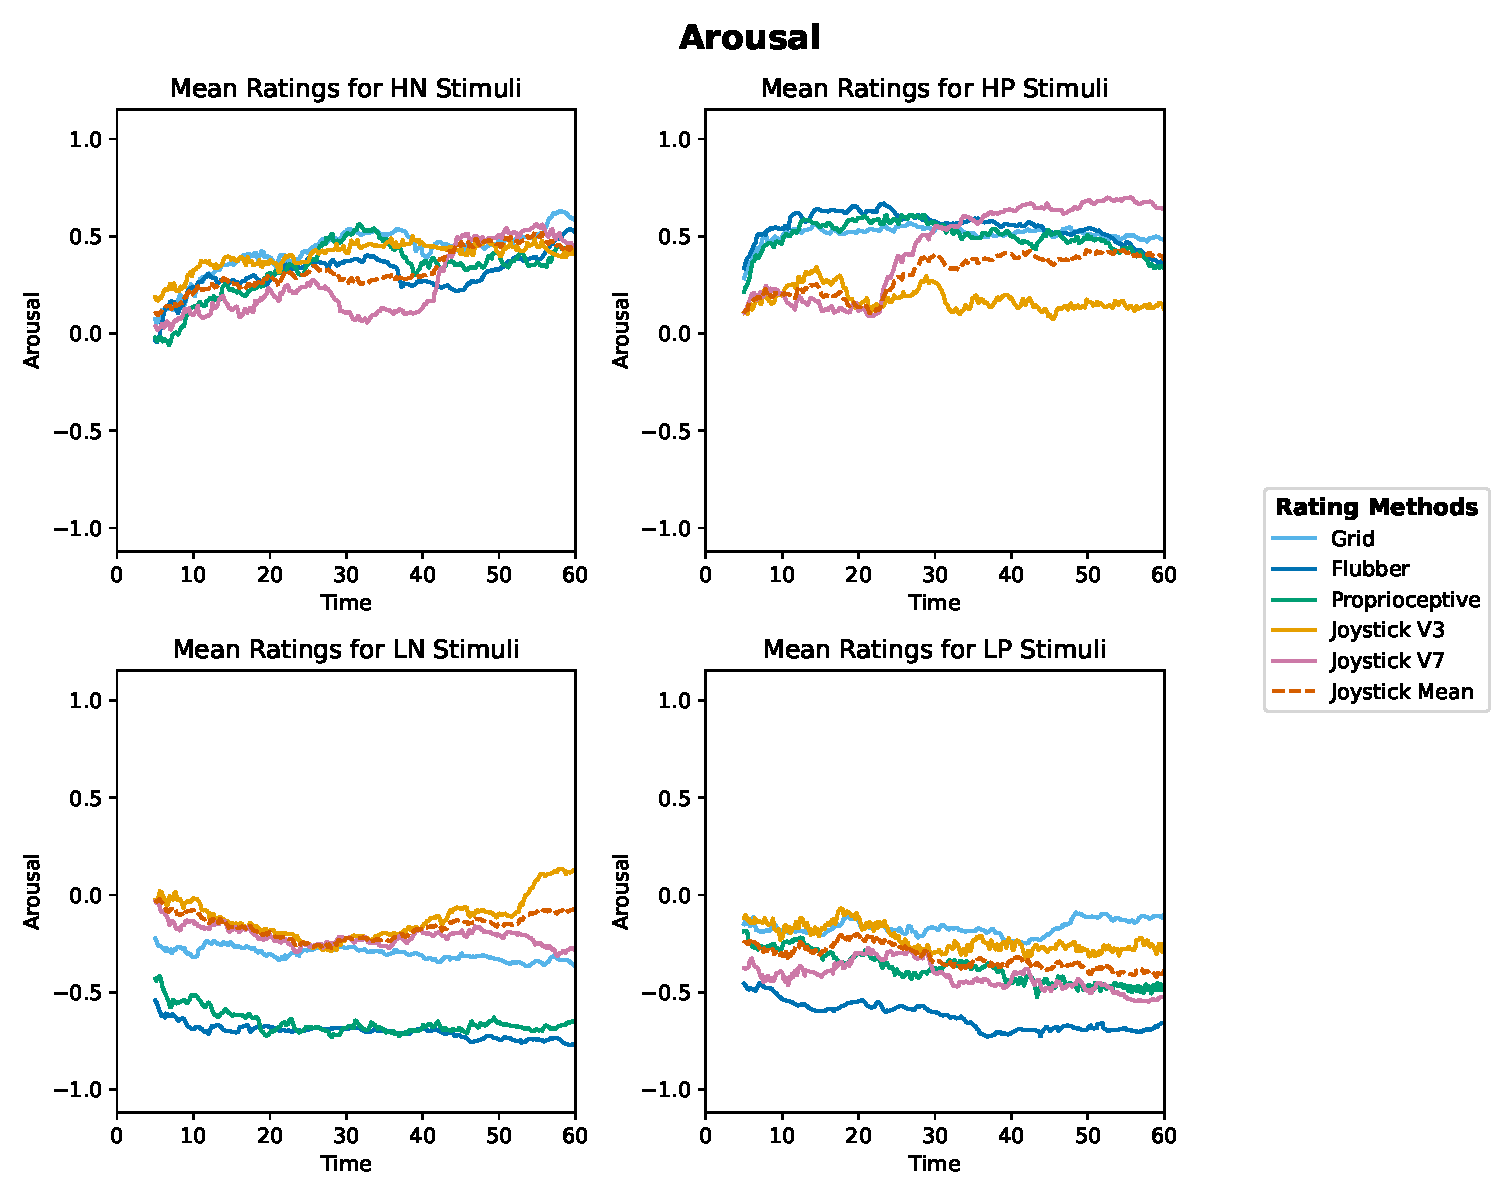
\includegraphics[width=\linewidth]{cr_a} 
        \caption{} \label{fig:cr_a}
    \end{subfigure}
    \hfill
    \begin{subfigure}[t]{0.49\textwidth}
        \centering
        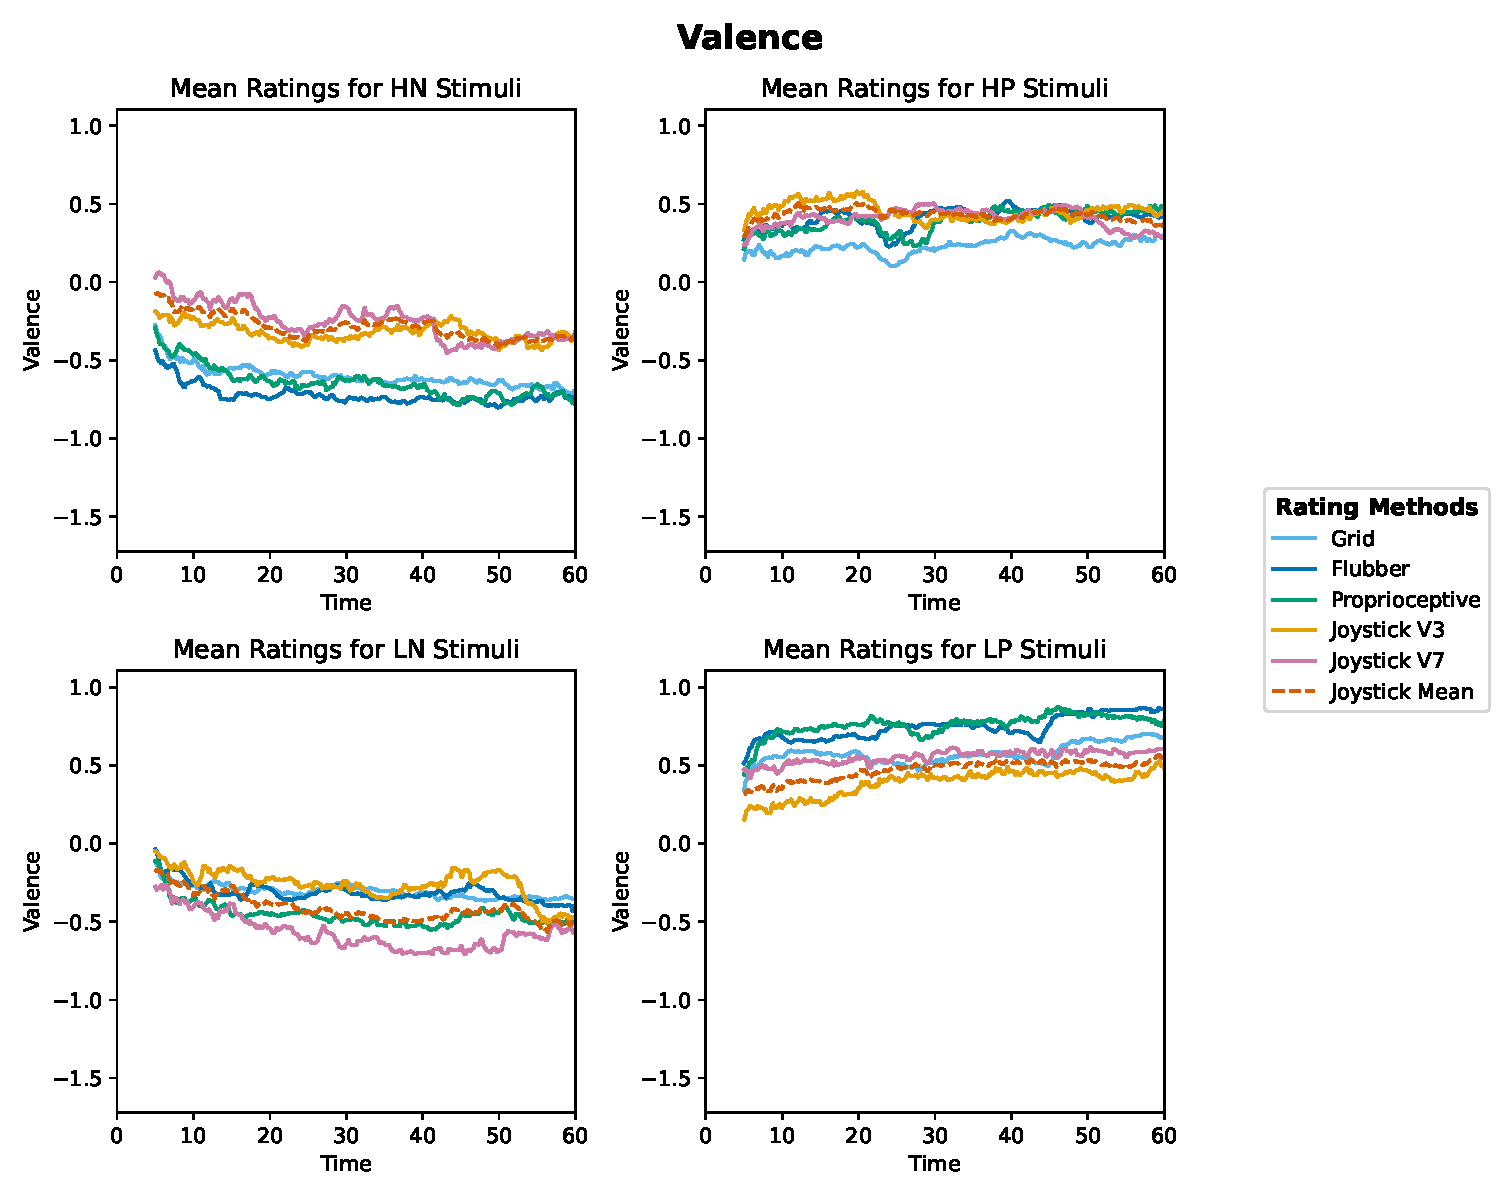
\includegraphics[width=\linewidth]{cr_v} 
        \caption{} \label{fig:cr_v}
    \end{subfigure}

    \vspace{1cm}
    \begin{subfigure}[t]{0.49\textwidth}
    \centering
        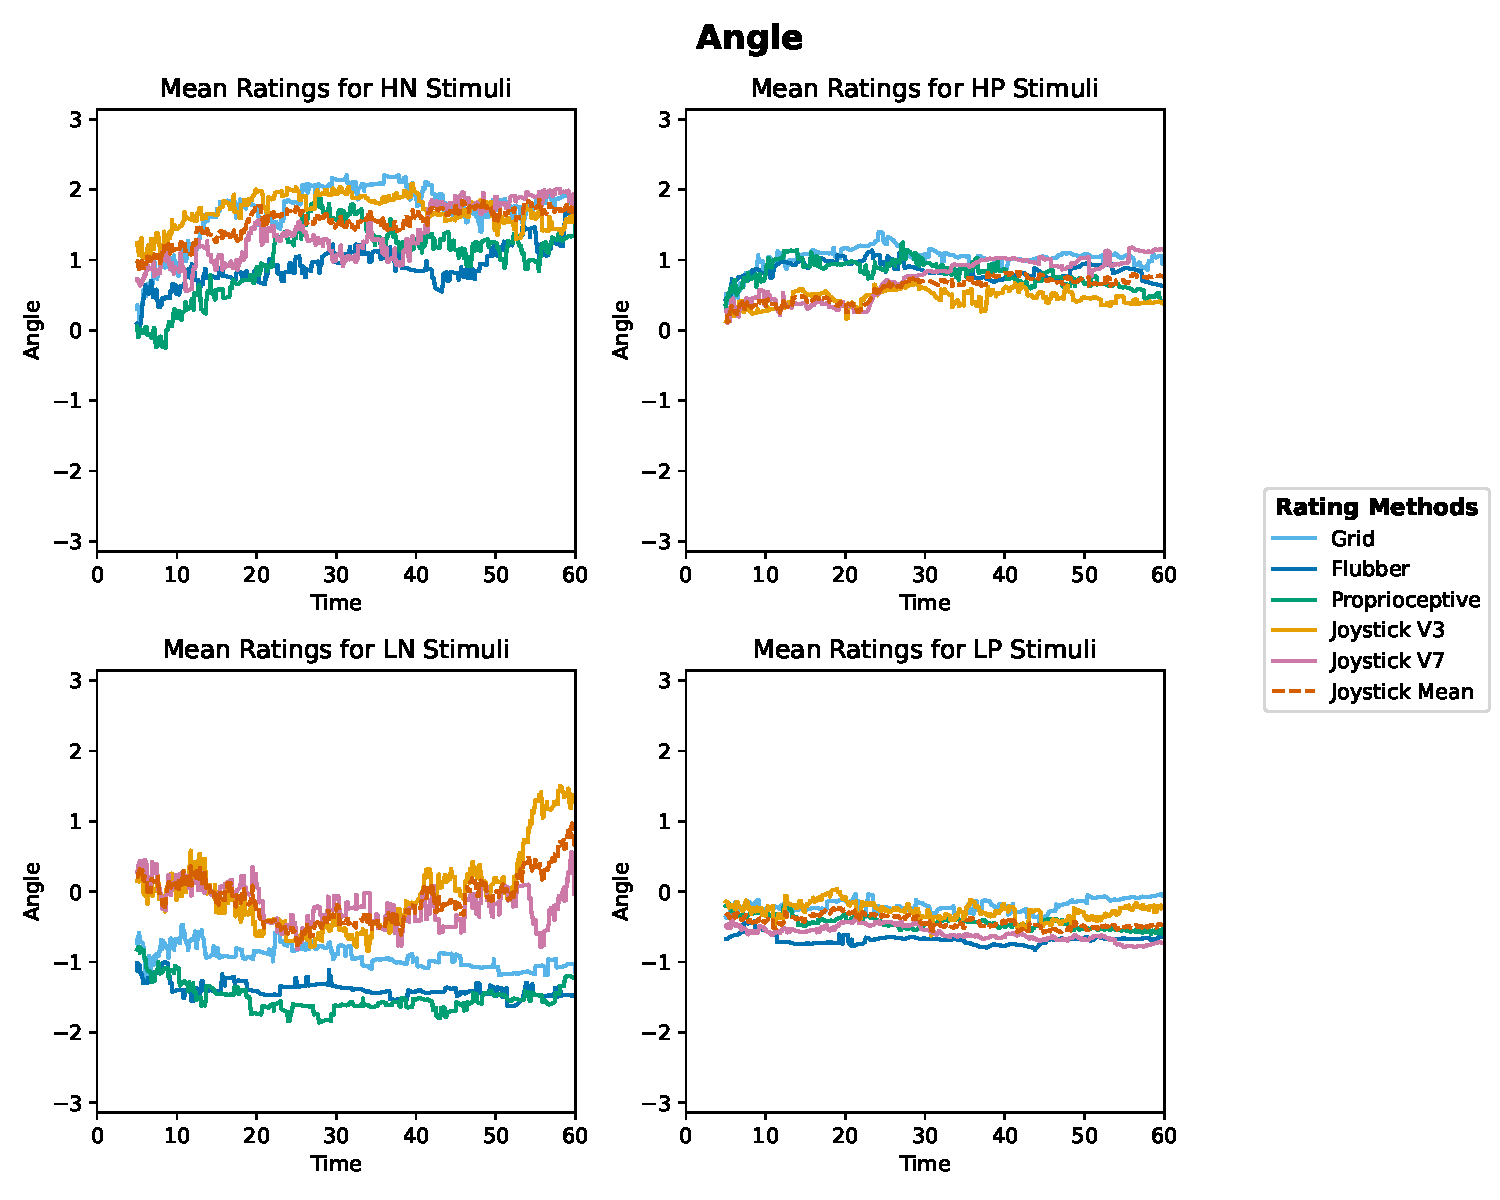
\includegraphics[width=\linewidth]{cr_angle} 
        \caption{} \label{fig:cr_angle}
    \end{subfigure}
    \hfill
    \begin{subfigure}[t]{0.49\textwidth}
    \centering
        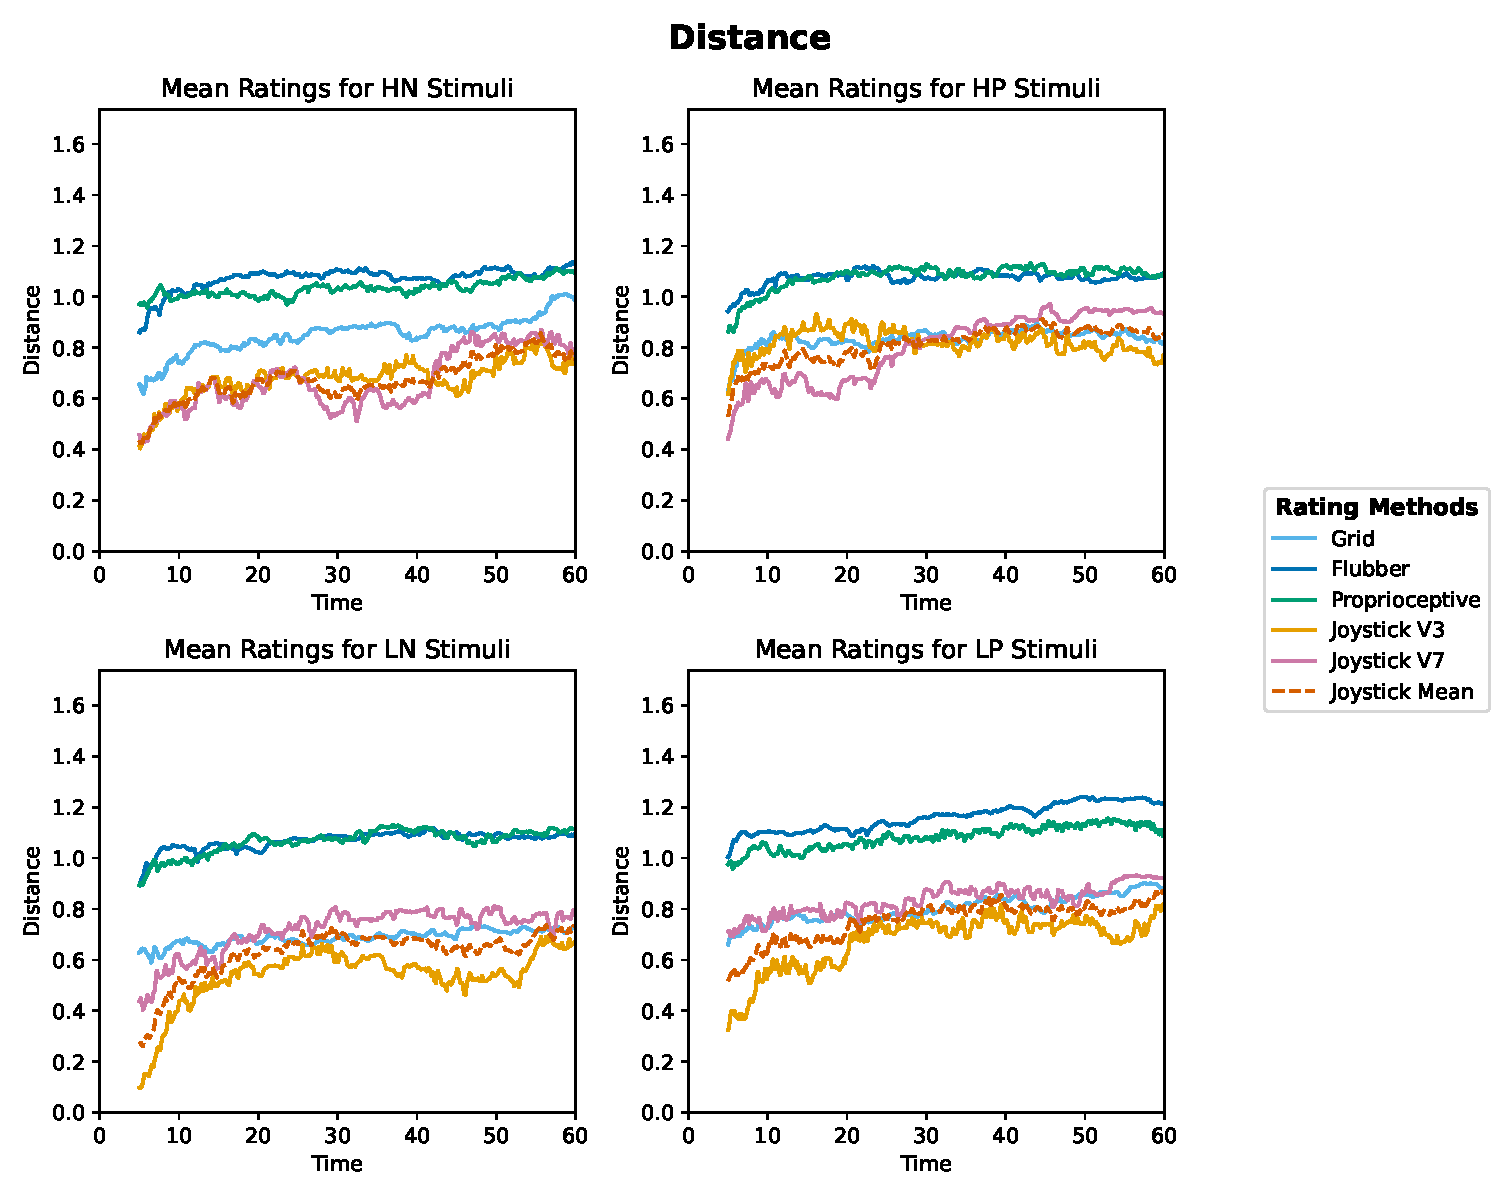
\includegraphics[width=\linewidth]{cr_dist} 
        \caption{} \label{fig:cr_dist}
    \end{subfigure}
    \caption{\textit{Mean ratings across four dimensions over time for different video categories and rating methods.} Affective VR data is depicted in blue colors, CEAP data is depicted in orange/pink colors. Ratings are similar for both datasets. (\subref{fig:cr_a}) Mean arousal ratings over time. (\subref{fig:cr_v}) Mean valence ratings over time. (\subref{fig:cr_angle}) Mean angle of arousal and valence ratings over time. (\subref{fig:cr_dist}) Mean distance of arousal and valence ratings over time. HN = highly negative stimuli (high arousal, low valence); HP = highly positive stimuli (high arousal, high valence); LN = low negative stimuli (low arousal, low valence); LP = low positive stimuli (low arousal, high valence).}
    \label{fig:mean_ratings}
\end{figure}

\newpage

% +++++ subsection arousal vs. valence ++++++
\subsection{Arousal vs. Valence}
Figure \ref{fig:mean_valence_arousal} shows the mean ratings of valence (x-axis) and arousal (y-axis) averaged over time and video categories for the different methods and datasets. Even though the means of both datasets vary, they are located in the same quadrant for each video category, respectively. Figure \ref{fig:valence_arousal}

% figure arousal vs. valence
\begin{figure}[h]
    \centering
    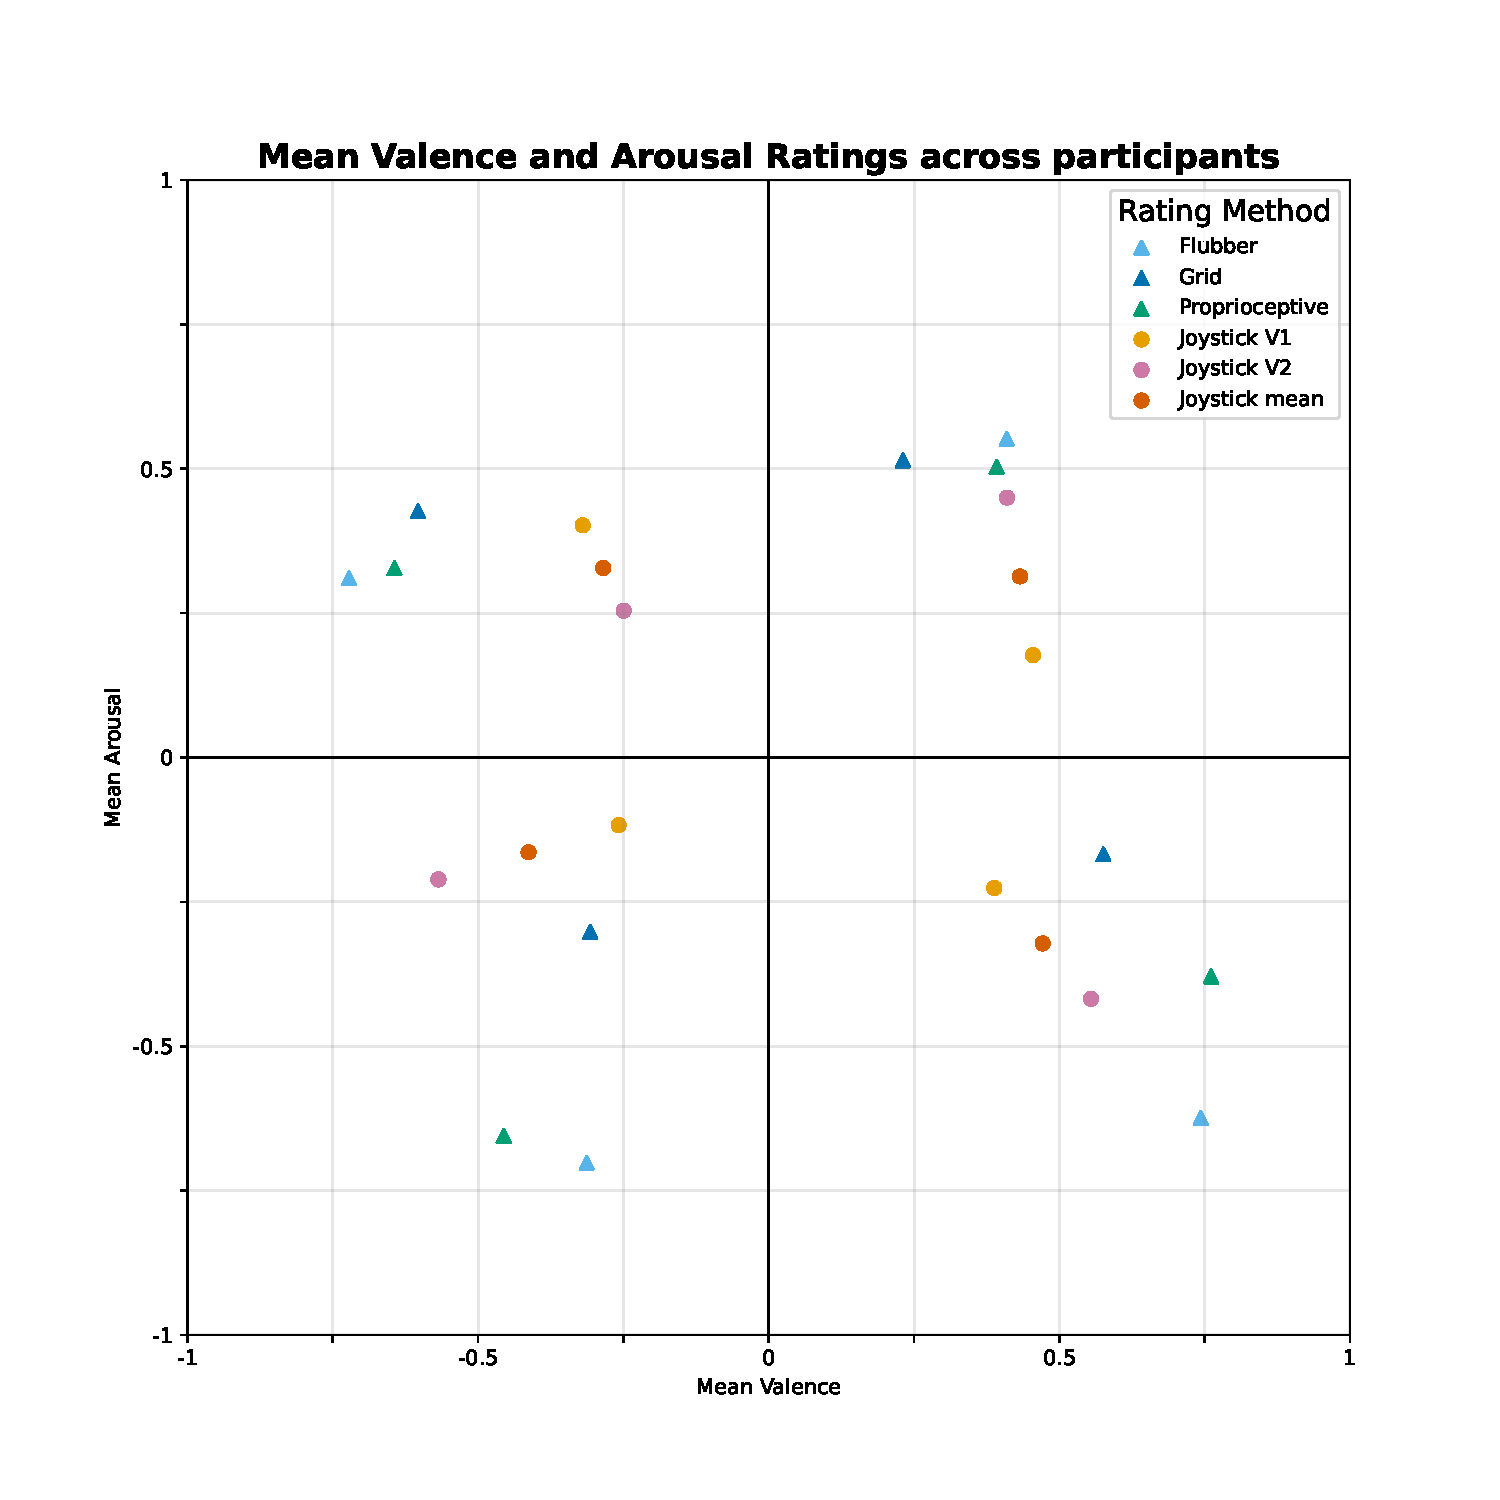
\includegraphics[width=0.99\textwidth]{mean_valence_arousal}
    \caption{\textit{Mean ratings of valence (x-axis) and arousal (y-axis) averaged over time and video categories for the different rating methods and datasets.} Affective VR data is depicted in blue colors (triangles), CEAP data is depicted in orange/pink colors (circles).}
    \label{fig:mean_valence_arousal}
\end{figure}

% figure arousal vs. valence for all timepoints
\begin{figure}
    \centering
    \begin{subfigure}[t]{0.49\textwidth}
        \centering
        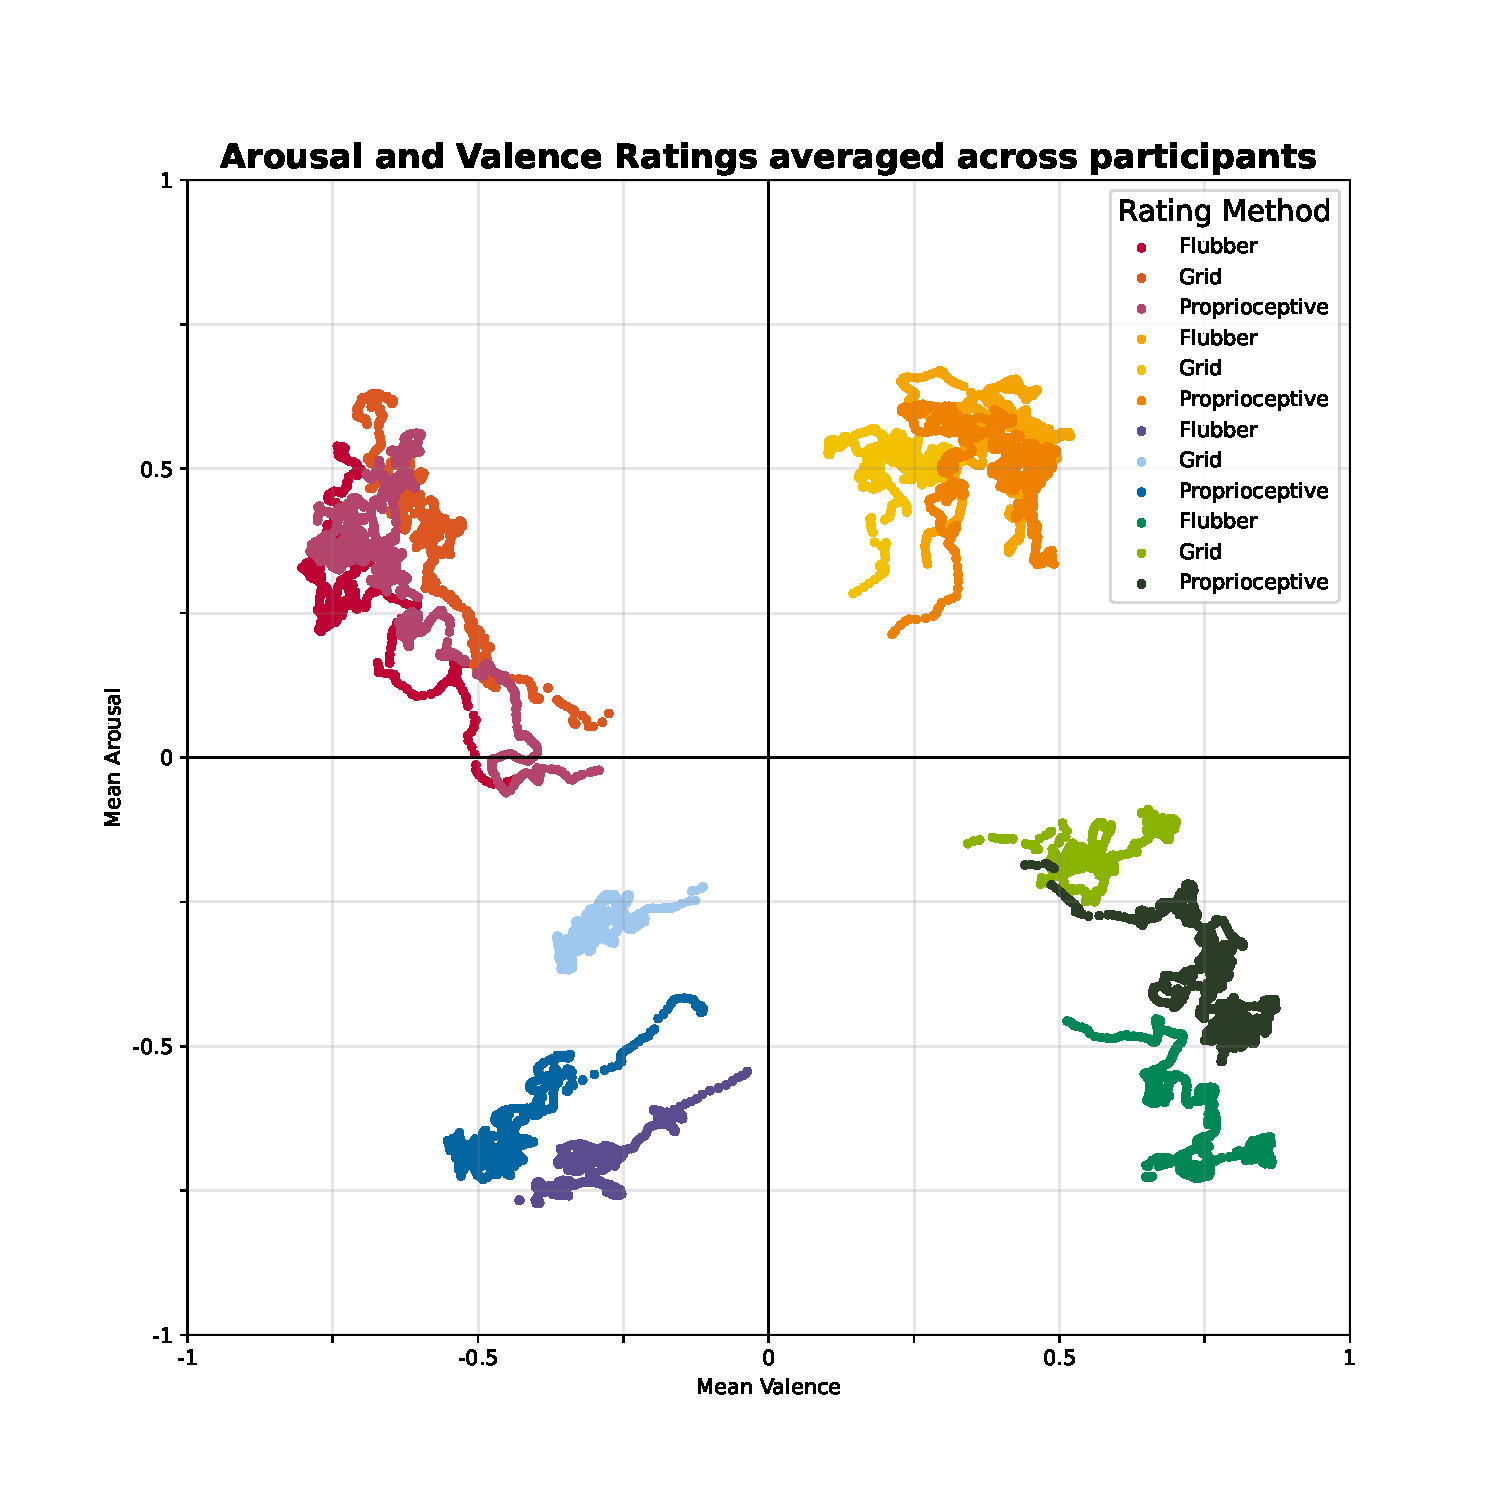
\includegraphics[width=\linewidth]{valence_arousal_affectivevr} 
        \caption{} \label{fig:valence_arousal_affectivevr}
    \end{subfigure}
    \hfill
    \begin{subfigure}[t]{0.49\textwidth}
        \centering
        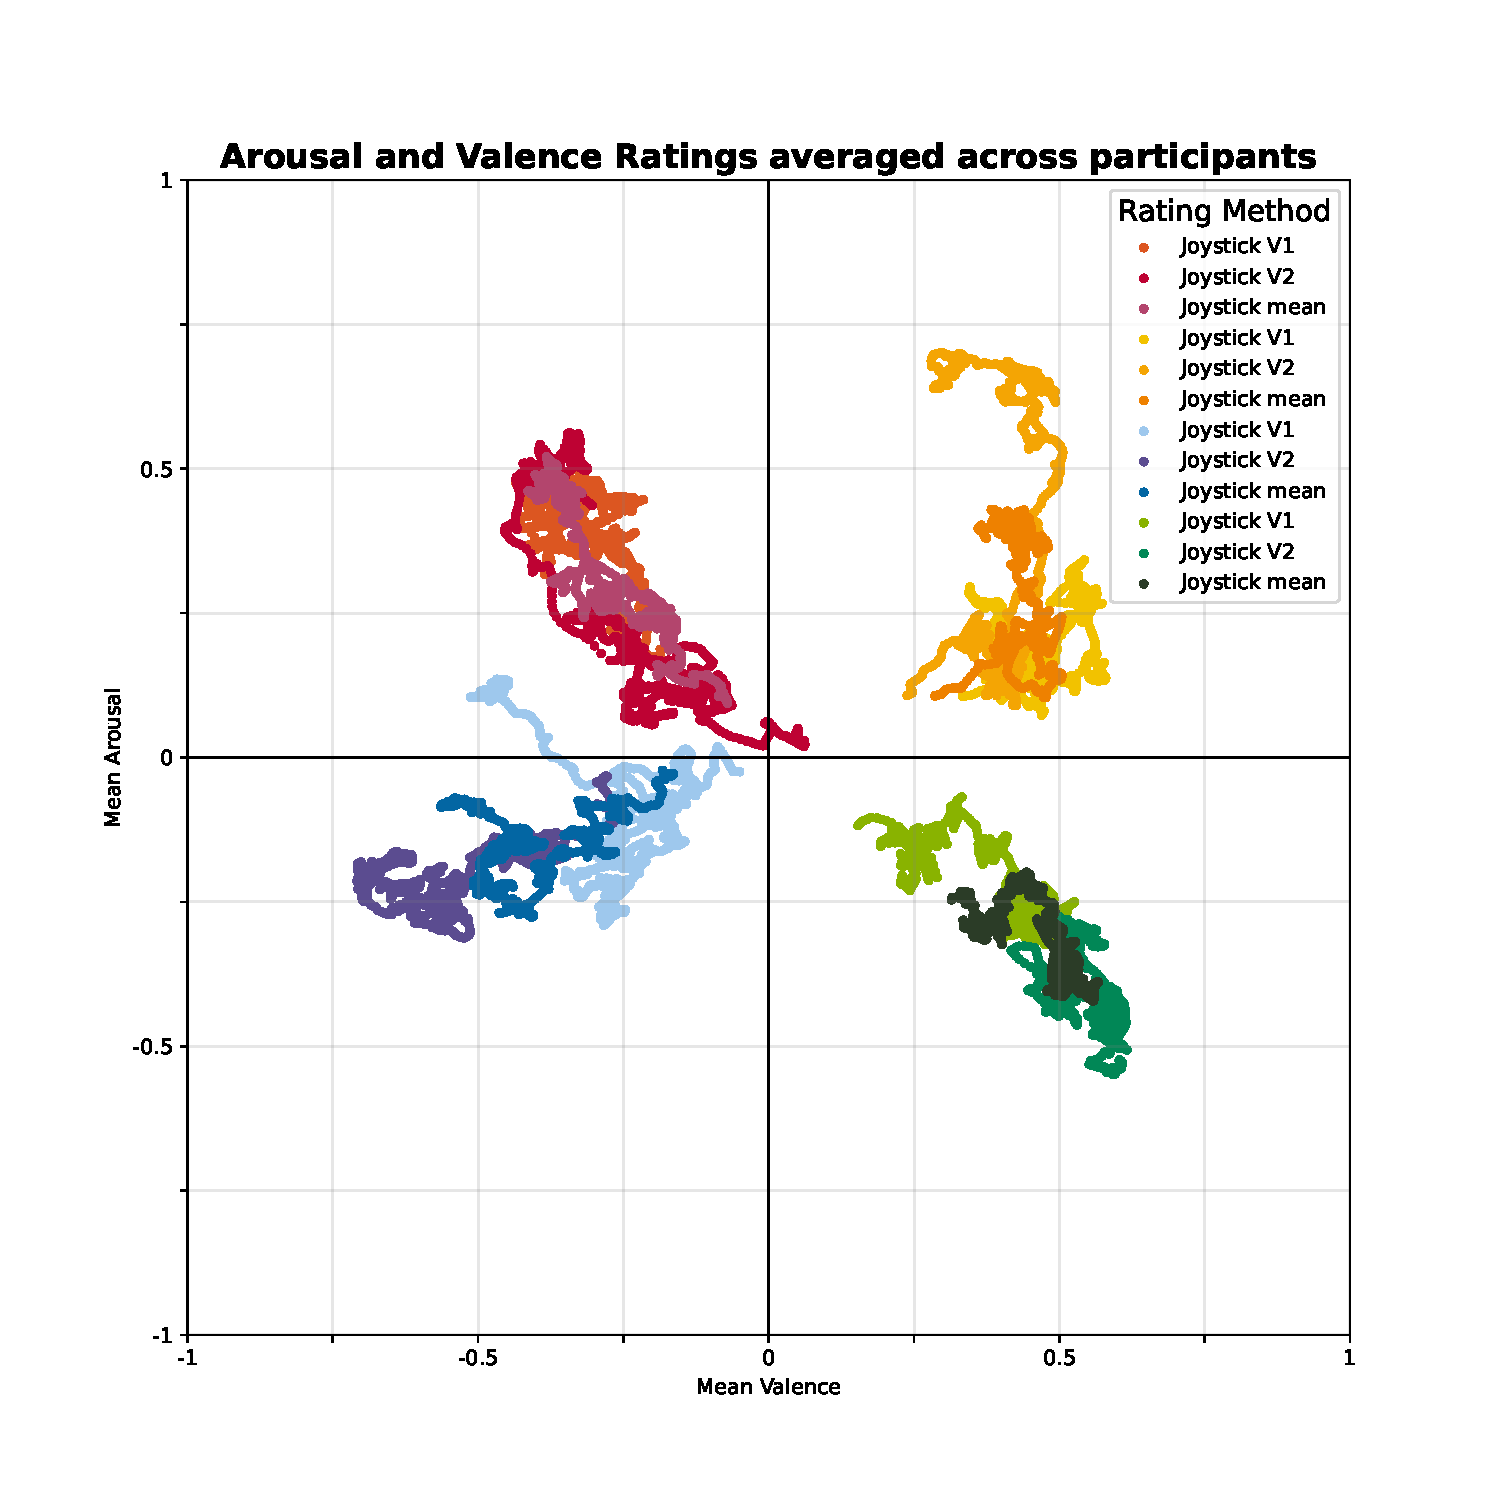
\includegraphics[width=\linewidth]{valence_arousal_ceap} 
        \caption{} \label{fig:valence_arousal_ceap}
    \end{subfigure}
    \caption{\textit{Ratings of valence (x-axis) and arousal (y-axis) for all timepoints for the different rating methods and datasets.} \subref{fig:valence_arousal_affectivevr} Affective VR data. \subref{fig:valence_arousal_affectivevr} CEAP data.}
    \label{fig:valence_arousal}
\end{figure}

\newpage
\newpage

% +++++ subsection summary statistics ++++++
\subsection{Summary Statistics}
A selection of the summary statistics of both datasets averaged across participants but for each video category separately can be found in Table \ref{tab:summary_stats_affectivevr} and \ref{tab:summary_stats_ceap}.

% table summary stats affectivevr
\begin{table}[H]
\centering
\caption{\textit{Summary Statistics of Affective VR dataset for the different rating methods and video categories.} Q = Quadrant (video category); M = Mean; STD = Standard Deviation.}
\label{tab:summary_stats_affectivevr}
\resizebox{\textwidth}{!}{%
\begin{tabular}{lccccccccc}
\hline
\textbf{Rating Method} & \textbf{Q} & \textbf{M Arousal} & \textbf{M Valence} & \textbf{M Angle} & \textbf{M Distance} & \textbf{STD Arousal} & \textbf{STD Valence} & \textbf{STD Angle} & \textbf{STD Distance} \\ \hline
Grid & HP & 0.51 & 0.23 & 1.03 & 0.84 & 0.36 & 0.57 & 1.02 & 0.28 \\
Grid & LP & -0.17 & 0.58 & -0.20 & 0.80 & 0.51 & 0.34 & 0.91 & 0.30 \\
Grid & LN & -0.30 &  & -0.93 & 0.69 & 0.46 & 0.39 & 1.99 & 0.28 \\
Grid & HN & 0.43 & -0.60 & 1.71 & 0.85 & 0.41 & 0.34 & 1.71 & 0.32 \\ \hline
Flubber & HP & 0.55 & 0.41 & 0.86 & 1.07 & 0.51 & 0.70 & 1.06 & 0.26 \\
Flubber & LP & -0.62 & 0.74 & -0.68 & 1.16 & 0.52 & 0.42 & 0.68 & 0.21 \\
Flubber & LN & -0.70 & -0.31 & -1.39 & 1.07 & 0.50 & 0.59 & 1.44 & 0.22 \\
Flubber & HN & 0.31 & -0.72 & 0.92 & 1.07 & 0.63 & 0.43 & 2.27 & 0.24 \\ \hline
Proprioceptive & HP & 0.50 & 0.39 & 0.81 & 1.08 & 0.54 & 0.73 & 1.17 & 0.24 \\
Proprioceptive & LP & -0.38 & 0.76 & -0.44 & 1.08 & 0.61 & 0.37 & 0.74 & 0.23 \\
Proprioceptive & LN & -0.66 & -0.46 & -1.51 & 1.07 & 0.50 & 0.58 & 1.50 & 0.28 \\
Proprioceptive & HN & 0.33 & -0.64 & 1.03 & 1.03 & 0.63 & 0.47 & 2.14 & \textit{0.27} \\ \hline
\end{tabular}%
}
\end{table}

% table summary stats ceap
\begin{table}[H]
\centering
\caption{\textit{Summary Statistics of CEAP dataset for the different rating methods and video categories.} Q = Quadrant (video category); M = Mean; STD = Standard Deviation.}
\label{tab:summary_stats_ceap}
\resizebox{\textwidth}{!}{%
\begin{tabular}{lccccccccc}
\hline
\textbf{Rating Method} & \textbf{Q} & \textbf{M Arousal} & \textbf{M Valence} & \textbf{M Angle} & \textbf{M Distance} & \textbf{STD Arousal} & \textbf{STD Valence} & \textbf{STD Angle} & \textbf{STD Distance} \\ \hline
V1 & HP & 0.18 & 0.45 & 0.46 & 0.82 & 0.48 & 0.60 & 1.03 & 0.39 \\
V1 & LP & -0.23 & 0.39 & -0.27 & 0.68 & 0.49 & 0.41 & 0.91 & 0.39 \\
V1 & HN & 0.40 & -0.32 & 1.70 & 0.68 & 0.37 & 0.45 & 1.21 & 0.38 \\
V1 & LN & -0.12 & -0.26 & -0.02 & 0.54 & 0.42 & 0.42 & 2.11 & 0.38 \\ \hline
V2 & HP & 0.45 & 0.41 & 0.74 & 0.80 & 0.48 & 0.40 & 0.86 & 0.33 \\
V2 & LP & -0.42 & 0.55 & -0.59 & 0.84 & 0.45 & 0.32 & 0.62 & 0.30 \\
V2 & HN & 0.25 & -0.25 & 1.37 & 0.67 & 0.43 & 0.55 & 1.52 & 0.40 \\
V2 & LN & -0.21 & -0.57 & -0.18 & 0.72 & 0.35 & 0.39 & 2.58 & 0.36 \\ \hline
Mean & HP & 0.31 & 0.43 & 0.60 & 0.81 & 0.50 & 0.51 & 0.96 & 0.36 \\
Mean & LP & -0.32 & 0.47 & -0.43 & 0.76 & 0.48 & 0.38 & 0.79 & 0.36 \\
Mean & LN & -0.16 & -0.41 & -0.10 & 0.63 & 0.39 & 0.43 & 2.36 & 0.38 \\
Mean & HN & 0.33 & -0.28 & 1.53 & 0.68 & 0.41 & 0.50 & 1.39 & 0.39 \\ \hline
\end{tabular}%
}
\end{table}

% ----------------------------------------------------- code and figure availability ---------------------------------------------------------------
\section{Code and Figure Availability} \label{code}
All python scripts can be found on GitHub: 
\url{https://github.com/lucyroe/CEAP_Analysis}.
All figures depicted here can also be found separately on OwnCloud in the AffectiveVR directory.

\end{document}